\chapter{Quantifying MGXS Approximations}
\label{chap:biases}

\begin{itemize}[noitemsep]
  \item stronger ending with summary
  \item remove redundant double precision compilation sentence
  \item detail flux-limited approx. for the transport corrected xs NOT the outscatter approx. (chap. 2)
  \begin{itemize}[noitemsep]
    \item the outscatter approx uses reversibility assumption to interchange energy indices in the scattering matrix
    \item our approximation weights with the scalar flux instead of J(E) (should be P(E)?)
  \end{itemize}
  \item Embolden/highlight bottom 70-group line in each table
  \item Add subsections/bold signposts to each case study
  \item mention that 1D slab and fuel pin are not equivalent
  \begin{itemize}
    \item need to preserve chord lengths and use isolated slab/pin rather than reflective
  \end{itemize}
\end{itemize}

As discussed in Chapter~\ref{chap:mgxs}, a number of approximations are made in the multi-group formulation of the neutron transport equation and the \ac{MGXS} generation process. These approximations remain even if one uses the ``true'' scalar flux for energy condensation and spatial homogenization, as is the case with energy condensation and spatial homogenization in Monte Carlo\footnote{By the Law of Large Numbers, the \ac{MC} flux will be exactly correct in the limit of an infinite number of particle histories, though it is only a ``noisy'' proxy for a finite number of particles.}. The observed bias between a continuous energy \ac{MC} and a multi-group deterministic calculation reflects the convolution of these approximations, which may (or may not) lead to some degree of fortuitous cancellation of error. Although this thesis is motivated by the need for \ac{MGXS} for whole core calculations, it is instructive to investigate the approximations inherent in multi-group theory and quantify their impact for simple benchmark models.

In this chapter, a series of case studies is devised to systematically quantify biases inherent to the energy condensation and spatial homogenization process in multi-group transport theory. The results underline the complex interactions between discretizations in energy, space and angle. Various convergence studies with respect to each of these variables are presented to quantify the resulting magnitude of the bias induced between continuous energy Monte Carlo and multi-group deterministic calculations. The results in this chapter illustrate the loss in accuracy resulting from scalar flux-weighted \ac{MGXS} and highlight the need for models of the angular dependency in \ac{MGXS} for fine-mesh deterministic neutron transport. Finally, this chapter verifies the data pipeline used to compute multi-group cross sections with OpenMC for use in OpenMOC.


%%%%%%%%%%%%%%%%%%%%%%%%%%%%%%%%%%%%%%%%%%%%%%%%%%%%%%%%%%%%%%%%%%%%%%%%%%%%%%%%
\section{Case Studies}
\label{sec:chap4-case-studies}

This chapter investigates the loss in accuracy resulting from approximations made in both the \ac{MOC} equations as well as the \ac{MGXS} generation scheme with OpenMC. The benchmarks are designed to illustrate the emergence of the approximation errors as increasing heterogeneity is introduced in the geometric models. The approximation errors are quantified for a variety of geometric and material configurations based on a standard \ac{PWR} . In each case, the bias $\Delta\rho$ compares the eigenvalue $k_{eff}^{OpenMOC}$ computed with \ac{MGXS} in OpenMOC to that of the reference eigenvalue $k_{eff}^{OpenMC}$ computed with continuous energy cross sections in OpenMC in units of \ac{PCM}:

\begin{equation}
\label{eqn:chap4-delta-rho}
\Delta\rho = \left(k_{eff}^{OpenMOC} - k_{eff}^{OpenMC}\right) \times 1E5
\end{equation}

In each case study, the role of angular discretization in \ac{MOC} is quantified through convergence studies of the number of azimuthal angles and the track spacing used in the deterministic calculations. The effects of energy discretization are analyzed for \ac{MGXS} tallied in the CASMO~\cite{rhodes2006casmo} energy group structures ranging from 1 -- 70 groups (see~\ref{app:energy-groups}). For each of the case studies with heterogeneous geometries, the spatial domain is discretized in OpenMOC's \ac{FSR} mesh with constant-by-material \ac{MGXS} to quantify the interaction between the energy and spatial approximations. Spatial discretization studies show the impact of tallying \ac{MGXS} in each of the \ac{FSR}s used in the discretized OpenMOC geometry. Finally, \ac{MGXS} libraries were tallied using OpenMC's ``iso-in-lab'' feature to quantify the impact of the isotropic in lab scattering approximation used in OpenMOC. Inter-pin spatial self-shielding effects are not treated here as they are studied in detail in subsequent chapters.

%%%%%%%%%%%%%%%%%%%%%%%%%%%%
\subsection{Homogeneous Infinite Medium}
\label{subsec:chap4-inf-medium}

An initial case study was performed for a homogeneous infinite medium problem. The isotopic composition of the infinite medium was constructed to mimic that of a homogenized \ac{PWR} pin cell and is described in Table~\ref{table:chap4-inf-med-isotopes}. No approximation is made in the multi-group formulation of the transport equation in the case of homogeneous infinite media. As a result, neutron balance should be exactly preserved within numerical precision in deterministic calculations with \ac{MGXS} computed in any energy group structure, assuming the tallies used to compute \ac{MGXS} are sufficiently converged.

\begin{table}[h!]
  \centering
  \caption[Infinite medium isotopic composition]{Homogeneous infinite medium isotopic composition.}
  \small
  \label{table:chap4-inf-med-isotopes} 
  \vspace{6pt}
  \begin{tabular}{a c}
  \toprule
  \rowcolor{lightgray}
  {\bf Nuclide} &
  {\bf Density [at/b-cm]} \\
  \midrule
  H-1 &   4.123778597552705E-2 \\
  O-16 &  2.062180312907649E-2 \\
  Zr-90 & 3.009046301354838E-3 \\
  U-235 & 1.623109453918422E-4 \\
  U-238 & 9.791980637067758E-3 \\
  \bottomrule
\end{tabular}
\end{table}

The reference eigenvalues computed with continuous energy cross sections in OpenMC are shown in Table~\ref{table:chap4-inf-med-reference} for both normal anisotropic as well as ``iso-in-lab'' scattering. As one would expect for a homogeneous infinite medium, the eigenvalues for anisotropic and ``iso-in-lab'' scattering match within statistics.  The reference calculations were computed for 100 batches of 1E8 particles per batch. The \texttt{openc.mgxs} module was used to compute 70-group libraries of $\Sigma^T_g$, $\nu\Sigma^F_g$, $\nu_s\Sigma^S_{gg'}$ and $\chi_g$ from OpenMC tallies. An installation of OpenMOC compiled with double precision floating point arithmetic was used for each deterministic simulation. In each calculation, OpenMOC was converged to a criterion of 1E-7 on the energy-integrated fission source.

\begin{table}[h!]
  \centering
  \caption[Reference $k^{OpenMC}_{\infty}$ for an infinite medium]{Reference $k^{OpenMC}_{\infty}$ for a homogeneous infinite medium.}
  \small
  \label{table:chap4-inf-med-reference} 
  \vspace{6pt}
  \begin{tabular}{c c}
  \toprule
  \rowcolor{lightgray}
  {\bf Anisotropic} &
  {\bf Isotropic in Lab} \\
  \midrule
  1.15908 $\pm$ 0.00001 & 1.15907 $\pm$ 0.00001 \\
  \bottomrule
\end{tabular}
\end{table}

Table~\ref{table:chap4-inf-med-angle} presents the bias $\Delta\rho$ between OpenMC and OpenMOC for a matrix of azimuthal angles and track spacings. The results for both normal and ``iso-in-lab'' scattering indicate consistent agreement of the eigenvalues computed by OpenMOC with OpenMC irregardless of track discretization.

\begin{table}[h!]
  \centering
  \caption[Angular discretization error for an infinite medium]{Convergence study of the eigenvalue bias $\Delta\rho$ with varying azimuthal angle quadratures and track spacings for a homogeneous infinite medium.}
  \small
  \label{table:chap4-inf-med-angle}
  \vspace{6pt}
  \begin{tabular}{a S[table-format=2.1] S[table-format=2.1] S[table-format=2.1] c S[table-format=2.1] S[table-format=2.1] S[table-format=2.1]} 
  \toprule
  \rowcolor{lightgray}
  & \multicolumn{7}{c}{\boldmath $\Delta\rho$ {\bf [pcm]}} \\
  \midrule
  \rowcolor{lightgray}
  {\bf \# Angles} &
  {\bf 0.1 cm} & 
  {\bf 0.01 cm} & 
  {\bf 0.001 cm} &
  &
  {\bf 0.1 cm} & 
  {\bf 0.01 cm} & 
  {\bf 0.001 cm} \\
  \midrule
  & \multicolumn{3}{c}{\cellcolor{carolinablue} \bf Anisotropic} &
  \multicolumn{1}{c}{} &
  \multicolumn{3}{c}{\cellcolor{lightgreen} \bf Isotropic in Lab} \\
  \cline{2-4} \cline{6-8}
4 & 1.3 & 1.3 & 1.3 & & -0.1 & -0.1 & -0.1 \\
8 & 1.3 & 1.3 & 1.3 & & -0.1 & -0.1 & -0.1 \\
16 & 1.3 & 1.3 & 1.3 & & -0.1 & -0.1 & -0.1 \\
32 & 1.3 & 1.3 & 1.3 & & -0.1 & -0.1 & -0.1 \\
64 & 1.3 & 1.3 & 1.3 & & -0.1 & -0.1 & -0.1 \\
128 & 1.3 & 1.3 & 1.3 & & -0.1 & -0.1 & -0.1 \\
  \bottomrule
\end{tabular}
\end{table}

Table~\ref{table:chap4-inf-med-energy} presents the bias $\Delta\rho$ between OpenMC and OpenMOC for a matrix of energy group structures and \ac{FSR} spatial discretizations. The OpenMOC calculations each used 128 azimuthal angles and 0.01 cm track spacing. Although the eigenvalues differ by approximately 10 pcm for 1 -- 2 groups, the OpenMOC eigenvalues match the eigenvalues computed analytically from the 1- and 2-group \ac{MGXS} to within 1 pcm. The small $\Delta\rho$ for few groups may be due to numerical roundoff error since the \ac{MGXS} library was tallied in 70 groups in OpenMC and condensed to the coarser group structures with downstream data processing.

\begin{table}[h!]
  \centering
  \caption[Energy discretization error for an infinite medium]{Convergence study of the eigenvalue bias $\Delta\rho$ with varying energy groups structures for a homogeneous infinite medium.}
  \small
  \label{table:chap4-inf-med-energy} 
  \vspace{6pt}
  \begin{tabular}{a S[table-format=2.1] S[table-format=2.1]}
  \toprule
  \rowcolor{lightgray}
  & \multicolumn{2}{c}{\boldmath $\Delta\rho$ {\bf [pcm]}} \\
  \midrule
  \rowcolor{lightgray}
  {\textbf{\# Groups}} &
  {\bf Anisotropic} &
  {\bf Isotropic in Lab} \\
  \midrule
1 & -11.1 & -10.5 \\
2 & -9.5 & -7.1 \\
4 & -0.1 & -0.5 \\
8 & 0.3 & -0.0 \\
16 & -0.2 & 0.5 \\
25 & 1.8 & 0.1 \\
40 & 1.6 & 0.1 \\
70 & 1.3 & -0.1 \\
  \bottomrule
\end{tabular}
\end{table}


%%%%%%%%%%%%%%%%%%%%
\subsection{1D Slab}
\label{subsec:chap4-slab}

A simple slab model was constructed to quantify approximation errors in a 1D heterogeneous geometry with spatial self-shielding. The slab model was constructed as an ``equivalent'' 1D model to the 1.6\% enriched UO$_2$ \ac{PWR} fuel pin in the \ac{BEAVRS} \ac{PWR} model~\cite{horelik2013beavrs}. The geometric configuration of UO$_2$ fuel, zirconium clad and water moderator is illustrated in Figure~\ref{fig:chap4-slab} and the dimensions for each material zone are shown in Table~\ref{table:chap4-slab-widths}. The width of each spatial region was chosen to preserve the volumetric fraction of each material in the slab with those in the corresponding 2D fuel pin. Reflective boundary conditions were applied to both left and right edges in the geometry. The isotopic composition of each material in the slab is identical to the \ac{BEAVRS} fuel pin and is itemized in Table~\ref{table:chap4-slab-isotopes}. 

\begin{figure}[h!]
\begin{subfigure}{\textwidth}
  \centering
  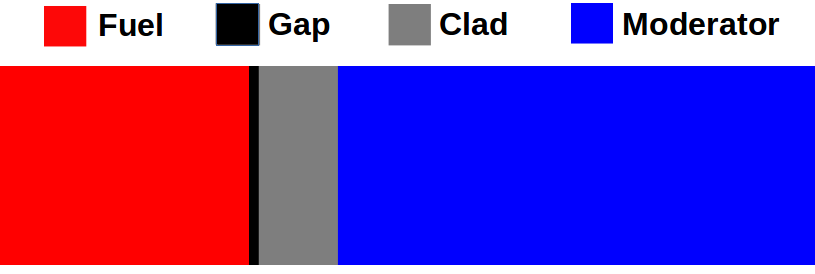
\includegraphics[width=0.7\linewidth]{figures/biases/slab/slab-simple-labels}
  \caption{}
\end{subfigure} \\
\begin{subfigure}{\textwidth}
  \centering
  
\includegraphics[width=0.7\linewidth]{figures/biases/slab/slab-8x}
  \caption{}
\end{subfigure}
\caption[1D slab materials and geometry]{A 1D slab with fuel, clad and moderator (a). Linearly-spaced tally zones were defined in the fuel and moderator in OpenMC and as \ac{FSR}s in OpenMOC (b).}
\label{fig:chap4-slab}
\end{figure}

\begin{table}[h!]
  \centering
  \caption[1D slab dimensions]{1D slab dimensions.}
  \small
  \label{table:chap4-slab-widths} 
  \vspace{6pt}
  \begin{tabular}{b c}
  \toprule
  \rowcolor{lightgray}
  \multicolumn{1}{c}{\bf Material} &
  \multicolumn{1}{c}{\bf Width [cm]} \\
  \midrule
  Fuel &  0.19177 \\
  Gap &   0.00777 \\
  Clad &  0.06109 \\
  Water & 0.36929 \\
  \bottomrule
\end{tabular}
\end{table}

\begin{table}[h!]
  \centering
  \caption[1D slab isotopic composition]{1D slab isotopic composition.}
  \small
  \label{table:chap4-slab-isotopes} 
  \vspace{6pt}
  \begin{tabular}{b c c}
  \toprule
  \rowcolor{lightgray}
  {\bf Material} &
  {\bf Nuclide} &
  {\bf Atom Density [at/b-cm]} \\
  \midrule
  \multirow{3}{*}{\bf UO$_2$} & O-16 &  4.5850826385693E-2 \\
  & U-235 & 5.5841582288888E-4 \\
  & U-238 & 2.2418671968636E-2 \\
  \midrule
  \multirow{1}{*}{\bf Helium} & He-4 & 2.40428068880973E-4 \\
  \midrule
  \multirow{3}{*}{\bf Zircaloy} & O-16 &  6.1404143720635E-4 \\
  & Fe-56 & 2.7183762028359E-4 \\
  & Zr-90 & 4.3595883452828E-2 \\
  \midrule
  \multirow{4}{*}{\bf Water} & H-1 &  4.95774559287053E-2 \\
  & B-10 & 8.02369478020388E-6 \\
  & B-11 & 3.22964691572685E-5 \\
  & O-16 & 2.47320903547125E-2 \\
  \bottomrule
\end{tabular}
\end{table}

The reference eigenvalues computed with continuous energy cross sections in OpenMC are shown in Table~\ref{table:chap4-slab-reference} for both normal anisotropic as well as ``iso-in-lab'' scattering. The reference calculations were computed for 100 batches of 1E7 particles per batch. The reference eigenvalues for the two cases vary by nearly 500 pcm due to anisotropies resulting from thermal scattering in the moderator. The \texttt{openc.mgxs} module was used to compute 70-group libraries of $\Sigma^T_g$, $\Sigma^{Tr}_g$, $\nu\Sigma^F_g$, $\nu_s\Sigma^S_{gg'}$ and $\chi_g$ from OpenMC tallies. An installation of OpenMOC compiled with double precision floating point arithmetic was used for each deterministic simulation. In each calculation, OpenMOC was converged to a criterion of 1E-7 on the energy-integrated fission source.

\begin{table}[h!]
  \centering
  \caption[Reference $k^{OpenMC}_{eff}$ for a 1D slab]{Reference $k^{OpenMC}_{eff}$ for a 1D slab.}
  \small
  \label{table:chap4-slab-reference} 
  \vspace{6pt}
  \begin{tabular}{c c}
  \toprule
  \rowcolor{lightgray}
  {\bf Anisotropic} &
  {\bf Isotropic in Lab} \\
  \midrule
  1.06513 $\pm$ 0.00003 & 1.05266 $\pm$ 0.00003 \\
  \bottomrule
\end{tabular}
\end{table}

Table~\ref{table:chap4-slab-angle} presents the bias $\Delta\rho$ between OpenMC and OpenMOC for a matrix of azimuthal angles and track spacings. No transport correction was applied to the total cross section $\Sigma^T_g$ or the scattering matrix $\nu_s\Sigma^S_{gg'}$. No spatial discretization was applied to the materials for the \ac{FSR} mesh in OpenMOC. The results for anisotropic and ``iso-in-lab'' scattering exhibit a bias resulting from the multi-group approximation which converges to 1200 and 1745 pcm, respectively. The magnitude of the bias appears to converge with 128 azimuthal angles and 0.01 cm spacing. The \ac{MGXS} tallied with ``iso-in-lab'' scattering in OpenMC eliminates the isotropic scattering approximation in OpenMOC but increases the overall bias by roughly 550 pcm with respect to the anisotropic case due to the cancellation of other approximation errors.

\begin{table}[h!]
  \centering
  \caption[Angular discretization error for a 1D slab]{Convergence study of the eigenvalue bias $\Delta\rho$ with varying azimuthal angle quadratures and track spacings for a 1D slab.}
  \small
  \label{table:chap4-slab-angle}
  \vspace{6pt}
  \begin{tabular}{a S[table-format=6.1] S[table-format=6.1] S[table-format=6.1] c S[table-format=6.1] S[table-format=6.1] S[table-format=6.1]} 
  \toprule
  \rowcolor{lightgray}
  & \multicolumn{7}{c}{\boldmath $\Delta\rho$ {\bf [pcm]}} \\
  \midrule
  \rowcolor{lightgray}
  {\bf \# Angles} &
  {\bf 0.1 cm} & 
  {\bf 0.01 cm} & 
  {\bf 0.001 cm} &
  &
  {\bf 0.1 cm} & 
  {\bf 0.01 cm} & 
  {\bf 0.001 cm} \\
  \midrule
  & \multicolumn{3}{c}{\cellcolor{carolinablue} \bf Anisotropic} &
  \multicolumn{1}{c}{} &
  \multicolumn{3}{c}{\cellcolor{lightgreen} \bf Isotropic in Lab} \\
4 & 5624 & 5265 & 5232 & & 6908 & 6549 & 6516 \\
8 & 4348 & 3902 & 3821 & & 5631 & 5185 & 5103 \\
16 & 3869 & 3381 & 3335 & & 5152 & 4663 & 4617 \\
32 & 3398 & 3305 & 3289 & & 4680 & 4586 & 4570 \\
64 & 3425 & 3297 & 3293 & & 4707 & 4578 & 4575 \\
128 & 3427 & 3293 & 3293 & & 4708 & 4575 & 4575 \\
256 & 3432 & 3294 & 3293 & & 4713 & 4575 & 4575 \\
512 & 3434 & 3293 & 3293 & & 4716 & 4575 & 4575 \\
%4 & 2338 & 2217 & 2203 & & 2885 & 2764 & 2750 \\
%8 & 1641 & 1455 & 1418 & & 2187 & 2000 & 1964 \\
%16 & 1463 & 1201 & 1177 & & 2009 & 1746 & 1721 \\
%32 & 1203 & 1180 & 1178 & & 1748 & 1725 & 1723 \\
%64 & 1218 & 1192 & 1197 & & 1763 & 1736 & 1742 \\
%128 & 1223 & 1198 & 1200 & & 1767 & 1743 & 1744 \\
%256 & 1224 & 1200 & 1200 & & 1769 & 1745 & 1745 \\
%512 & 1223 & 1200 & 1201 & & 1768 & 1744 & 1745 \\
  \bottomrule
\end{tabular}
\end{table}

Table~\ref{table:chap4-slab-energy} presents the bias $\Delta\rho$ between OpenMC and OpenMOC for a matrix of energy group structures and \ac{FSR} spatial discretizations. In each case, the \ac{MGXS} used in OpenMOC were tallied by material in OpenMC. The OpenMOC calculations each used 128 azimuthal angles and 0.05 cm track spacing. The slab was discretized into 1 -- 16 equal volume \ac{FSR}s in the fuel and moderator.

\begin{itemize}[noitemsep]
  \item refer back to figure (a) and (b) for energy/space table
\end{itemize}

\begin{table}[h!]
  \centering
  \caption[Energy and spatial discretization error for a 1D slab]{Convergence study of the eigenvalue bias $\Delta\rho$ with varying energy groups structures and \ac{FSR} spatial discretizations for a 1D slab with \textit{\ac{MGXS} tallied by material}.}
  \small
  \label{table:chap4-slab-energy} 
  \vspace{6pt}
  \begin{tabular}{a S[table-format=6.1] S[table-format=6.1] S[table-format=6.1] S[table-format=6.1] S[table-format=6.1]}
  \toprule
  \rowcolor{lightgray}
  & \multicolumn{5}{c}{\boldmath $\Delta\rho$ {\bf [pcm]}} \\
  \midrule
  \rowcolor{lightgray}
  {\textbf{\# Groups}} &
  {\bf 1$\times$} &
  {\bf 2$\times$} &
  {\bf 4$\times$} &
  {\bf 8$\times$} &
  {\bf 16$\times$} \\
  \midrule
  \multicolumn{6}{c}{\cellcolor{carolinablue} \bf Anisotropic $\left(\Sigma^T_g\right)$} \\
1 & 1215 & 1295 & 1342 & 1359 & 1364 \\
2 & 2265 & 922 & -213 & -712 & -872 \\
4 & 2362 & 980 & -199 & -718 & -890 \\
8 & 2980 & 1294 & -246 & -956 & -1197 \\
16 & 3164 & 1423 & -200 & -961 & -1221 \\
25 & 3159 & 1436 & -180 & -940 & -1200 \\
40 & 3259 & 1501 & -168 & -960 & -1233 \\
70 & 3293 & 1526 & -159 & -963 & {\cellcolor{darktangerine}} -1242 \\
%1 & 459 & 473 & 480 & 482 & 482 \\
%2 & 789 & 183 & -214 & -367 & -412 \\
%4 & 802 & 212 & -181 & -334 & -385 \\
%8 & 1067 & 271 & -298 & -527 & -604 \\
%16 & 1156 & 313 & -304 & -555 & -639 \\
%25 & 1129 & 307 & -299 & -547 & -633 \\
%40 & 1173 & 326 & -308 & -570 & -661 \\
%70 & 1191 & 336 & -309 & -577 & {\cellcolor{darktangerine}} -670 \\
  \multicolumn{6}{c}{\cellcolor{lightgreen} \bf Anisotropic $\left(\Sigma^{Tr}_g\right)$} \\
1 & 1126 & 1165 & 1185 & 1191 & 1192 \\
2 & 2620 & 1624 & 915 & 634 & 551 \\
4 & 2556 & 1516 & 778 & 484 & 386 \\
8 & 3135 & 1766 & 681 & 220 & 65 \\
16 & 3325 & 1898 & 727 & 214 & 40 \\
25 & 3262 & 1837 & 666 & 146 & -23 \\
40 & 3350 & 1888 & 664 & 111 & -71 \\
70 & 3384 & 1910 & 667 & 101 & {\cellcolor{darktangerine}} -86 \\
%1 & 404 & 410 & 413 & 413 & 413 \\
%2 & 1113 & 716 & 488 & 406 & 385 \\
%4 & 932 & 526 & 291 & 206 & 169 \\
%8 & 1151 & 533 & 140 & -10 & -68 \\
%16 & 1243 & 575 & 133 & -39 & -104 \\
%25 & 1130 & 467 & 26 & -152 & -210 \\
%40 & 1162 & 470 & 1 & -191 & -255 \\
%70 & 1178 & 476 & -6 & -204 & {\cellcolor{darktangerine}} -270 \\
  \multicolumn{6}{c}{\cellcolor{lightsalmonpink} \bf Isotropic in Lab $\left(\Sigma^T_g\right)$} \\
1 & 1464 & 1548 & 1598 & 1617 & 1622 \\
2 & 3660 & 2305 & 1159 & 654 & 493 \\
4 & 3619 & 2228 & 1040 & 517 & 343 \\
8 & 4339 & 2648 & 1103 & 390 & 149 \\
16 & 4516 & 2770 & 1143 & 380 & 120 \\
25 & 4456 & 2731 & 1112 & 352 & 91 \\
40 & 4544 & 2785 & 1115 & 323 & 49 \\
70 & 4575 & 2806 & 1120 & 316 & {\cellcolor{darktangerine}} 37 \\
%1 & 585 & 599 & 606 & 609 & 609 \\
%2 & 1467 & 856 & 455 & 300 & 254 \\
%4 & 1352 & 757 & 360 & 206 & 154 \\
%8 & 1686 & 887 & 316 & 86 & 9 \\
%16 & 1778 & 932 & 313 & 61 & -23 \\
%25 & 1686 & 863 & 255 & 7 & -79 \\
%40 & 1721 & 873 & 239 & -24 & -115 \\
%70 & 1735 & 879 & 234 & -34 & {\cellcolor{darktangerine}} -127 \\
  \bottomrule
\end{tabular}
\end{table}

The results illustrate a strong interaction between the energy and spatial meshes used to solve the multi-group transport equation. The eigenvalue bias varies by over 1000 pcm between energy group structures and nearly 2000 pcm between \ac{FSR} discretizations. The application of the transport correction reduces the bias by 400 pcm for the 70-group structure and 16$\times$ \ac{FSR} discretization. The use of the ``iso-in-lab'' scattering feature reduces the bias by 550 pcm with respect to anisotropic scattering. 

Table~\ref{table:chap4-slab-space} presents the bias $\Delta\rho$ for a matrix of energy group structures and \ac{MGXS} spatial tally zone meshes. In each case, the \ac{MGXS} were tallied on the \ac{FSR} mesh with 1 -- 16 equal volume subdivisions in the fuel and moderator. The OpenMOC calculations each used 128 azimuthal angles and 0.05 cm track spacing.

\begin{table}[h!]
  \centering
  \caption[Spatial homogenization error for a 1D slab]{Convergence study of the eigenvalue bias $\Delta\rho$ with varying energy groups structures and \ac{FSR} spatial discretizations for a 1D slab with \textit{\ac{MGXS} tallied by \ac{FSR}}.}
  \small
  \label{table:chap4-slab-space} 
  \vspace{6pt}
  \begin{tabular}{a S[table-format=6.1] S[table-format=6.1] S[table-format=6.1] S[table-format=6.1] S[table-format=6.1]}
  \toprule
  \rowcolor{lightgray}
  & \multicolumn{5}{c}{\boldmath $\Delta\rho$ {\bf [pcm]}} \\
  \midrule
  \rowcolor{lightgray}
  {\textbf{\# Groups}} &
  {\bf 1$\times$} &
  {\bf 2$\times$} &
  {\bf 4$\times$} &
  {\bf 8$\times$} &
  {\bf 16$\times$} \\
  \midrule
  \multicolumn{6}{c}{\cellcolor{carolinablue} \bf Anisotropic $\left(\Sigma^T_g\right)$} \\
1 & 1217 & 1351 & 1390 & 1431 & 1398 \\
2 & 2268 & 918 & -230 & -704 & -892 \\
4 & 2365 & 1023 & -105 & -599 & -769 \\
8 & 2982 & 1290 & -249 & -944 & -1187 \\
16 & 3167 & 1408 & -217 & -970 & -1236 \\
25 & 3161 & 1427 & -191 & -939 & -1202 \\
40 & 3261 & 1497 & -171 & -953 & -1228 \\
70 & 3296 & 1525 & -158 & -950 & {\cellcolor{darktangerine}} -1228 \\
%1 & 452 & 472 & 448 & 495 & 454 \\
%2 & 782 & 170 & -233 & -354 & -437 \\
%4 & 795 & 231 & -131 & -260 & -333 \\
%8 & 1060 & 267 & -288 & -504 & -596 \\
%16 & 1149 & 306 & -300 & -540 & -636 \\
%25 & 1122 & 305 & -294 & -530 & -616 \\
%40 & 1166 & 326 & -300 & -552 & -643 \\
%70 & 1184 & 339 & -298 & -558 & {\cellcolor{darktangerine}} -648 \\
  \multicolumn{6}{c}{\cellcolor{lightgreen} \bf Anisotropic $\left(\Sigma^{Tr}_g\right)$} \\
1 & 1129 & 1201 & 1230 & 1253 & 1244 \\
2 & 2623 & 1635 & 949 & 692 & 608 \\
4 & 2559 & 1577 & 892 & 634 & 539 \\
8 & 3138 & 1764 & 689 & 244 & 86 \\
16 & 3328 & 1886 & 709 & 205 & 26 \\
25 & 3265 & 1826 & 649 & 139 & -34 \\
40 & 3353 & 1882 & 653 & 109 & -78 \\
70 & 3387 & 1907 & 663 & 105 & {\cellcolor{darktangerine}} -88 \\
%1 & 397 & 419 & 439 & 449 & 444 \\
%2 & 1106 & 728 & 527 & 451 & 429 \\
%4 & 925 & 555 & 358 & 282 & 248 \\
%8 & 1144 & 533 & 158 & 14 & -44 \\
%16 & 1236 & 566 & 137 & -33 & -98 \\
%25 & 1123 & 451 & 20 & -155 & -212 \\
%40 & 1155 & 454 & -8 & -199 & -262 \\
%70 & 1171 & 461 & -13 & -211 & {\cellcolor{darktangerine}} -276 \\
  \multicolumn{6}{c}{\cellcolor{lightsalmonpink} \bf Isotropic in Lab $\left(\Sigma^T_g\right)$} \\
1 & 1466 & 1622 & 1692 & 1682 & 1686 \\
2 & 3662 & 2264 & 1123 & 601 & 451 \\
4 & 3621 & 2261 & 1116 & 625 & 464 \\
8 & 4341 & 2637 & 1094 & 383 & 144 \\
16 & 4518 & 2751 & 1118 & 352 & 93 \\
25 & 4458 & 2715 & 1097 & 341 & 82 \\
40 & 4547 & 2776 & 1110 & 322 & 49 \\
70 & 4577 & 2799 & 1118 & 318 & {\cellcolor{darktangerine}} 39 \\
%1 & 585 & 608 & 589 & 589 & 590 \\
%2 & 1467 & 852 & 449 & 272 & 238 \\
%4 & 1352 & 786 & 421 & 261 & 218 \\
%8 & 1686 & 894 & 334 & 92 & 20 \\
%16 & 1777 & 932 & 318 & 55 & -26 \\
%25 & 1685 & 863 & 251 & 3 & -77 \\
%40 & 1721 & 873 & 236 & -25 & -110 \\
%70 & 1735 & 881 & 235 & -32 & {\cellcolor{darktangerine}} -122 \\
  \bottomrule
\end{tabular}
\end{table}

The trends analyzed in Table~\ref{table:chap4-slab-energy} emerge in a nearly identical manner with spatially-dependent \ac{MGXS} in Table~\ref{table:chap4-slab-energy}. In particular, the eigenvalue bias grows in magnitude with more energy groups, and is largely invariant to \ac{FSR} spatial discretization or the elimination of the isotropic scattering approximation with ``iso-in-lab'' scattering. Most importantly, the results in Table~\ref{table:chap4-slab-space} indicate that spatial self-shielding effects (\textit{e.g.}, variations in the flux energy spectrum across the fuel) captured with spatially-varying scalar flux-weighted \ac{MGXS} for each \ac{FSR} do not have a substantial impact on the systematic errors in the eigenvalue for this 1D slab problem.


%%%%%%%%%%%%%%%%%%%%%%%%%%%%%
\subsection{2D Fuel Pin Cell}
\label{subsec:chap4-pin}

A \ac{PWR} fuel pin cell model was constructed to quantify approximation errors in a 2D heterogeneous geometry with spatial self-shielding. The pin cell is identical to the 1.6\% enriched UO$_2$ \ac{PWR} fuel pin in the \ac{BEAVRS} \ac{PWR} model~\cite{horelik2013beavrs}. The geometric configuration of UO$_2$ fuel, helium gap, zirconium clad and water moderator is illustrated in Figure~\ref{fig:chap4-pin-cell} and the dimensions for each material zone are shown in Table~\ref{table:chap4-pin-dimensions}. Reflective boundary conditions were applied to all edges in the geometry. The isotopic compositions of each material in the fuel pin were identical to those used in the 1D slab (see Table~\ref{table:chap4-slab-isotopes}). 

\begin{table}[H]
  \centering
  \caption[2D fuel pin dimensions]{2D fuel pin dimensions.}
  \label{table:chap4-pin-dimensions} 
  \vspace{6pt}
  \begin{tabular}{b c}
  \toprule
  \rowcolor{lightgray}
  {\bf Material} &
  {\bf Dimension [cm]} \\
  \midrule
  Fuel Outer Radius &     0.39218 \\
  Gap Outer Radius &      0.40005 \\
  Clad Outer Radius &     0.45720 \\
  Pin Pitch &             1.25984 \\
  \bottomrule
\end{tabular}
\end{table}

\begin{figure}[H]
\centering
\begin{subfigure}{.32\textwidth}
  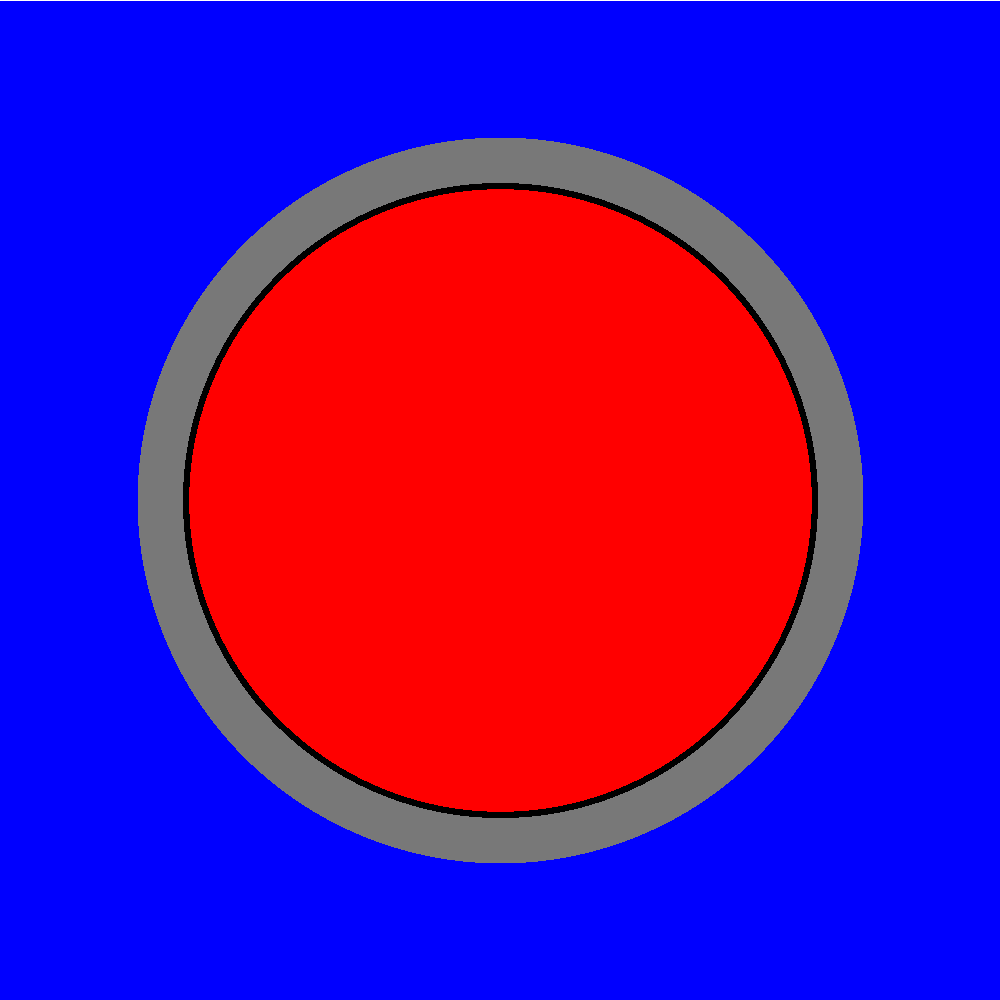
\includegraphics[width=0.9\linewidth]{figures/biases/pin-cell/pin-cell-simple}
  \caption{}
\end{subfigure}%
\begin{subfigure}{.32\textwidth}
  \centering
  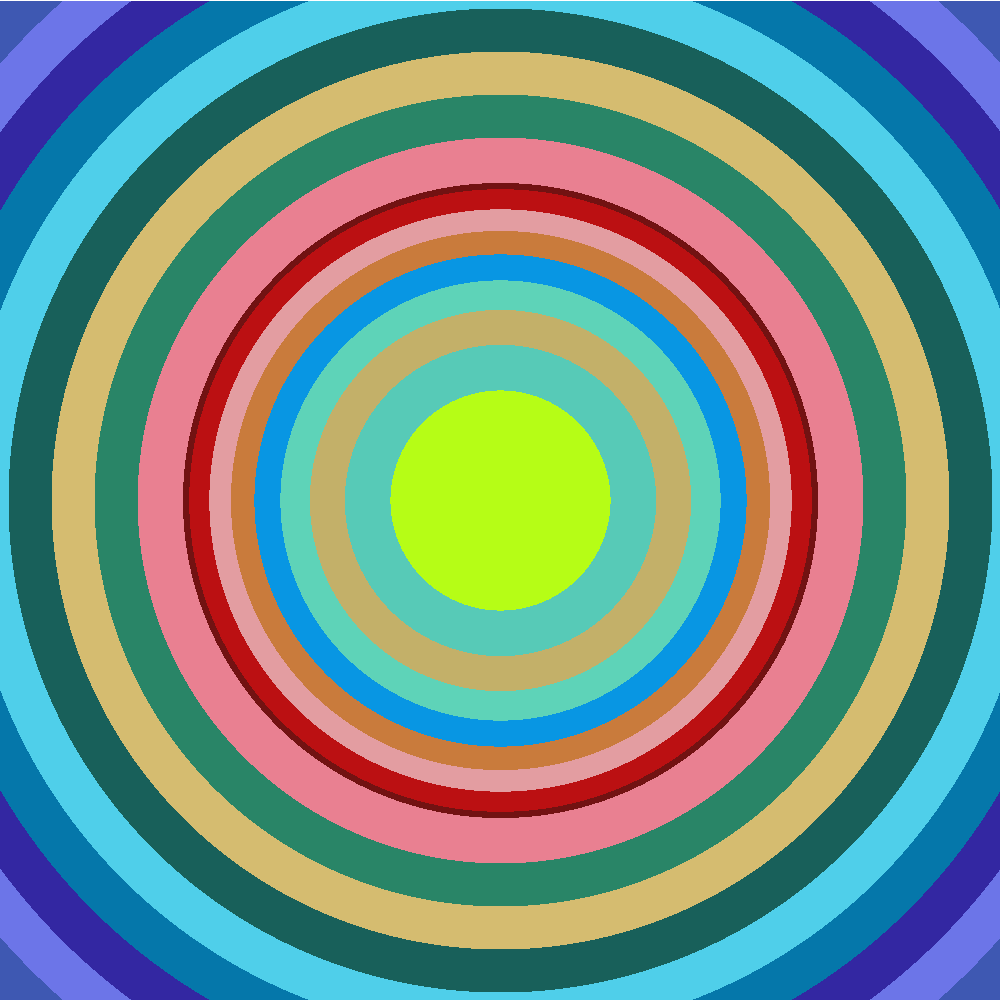
\includegraphics[width=0.9\linewidth]{figures/biases/pin-cell/pin-cell-8x}
  \caption{}
\end{subfigure}
\begin{subfigure}{.32\textwidth}
  \centering
  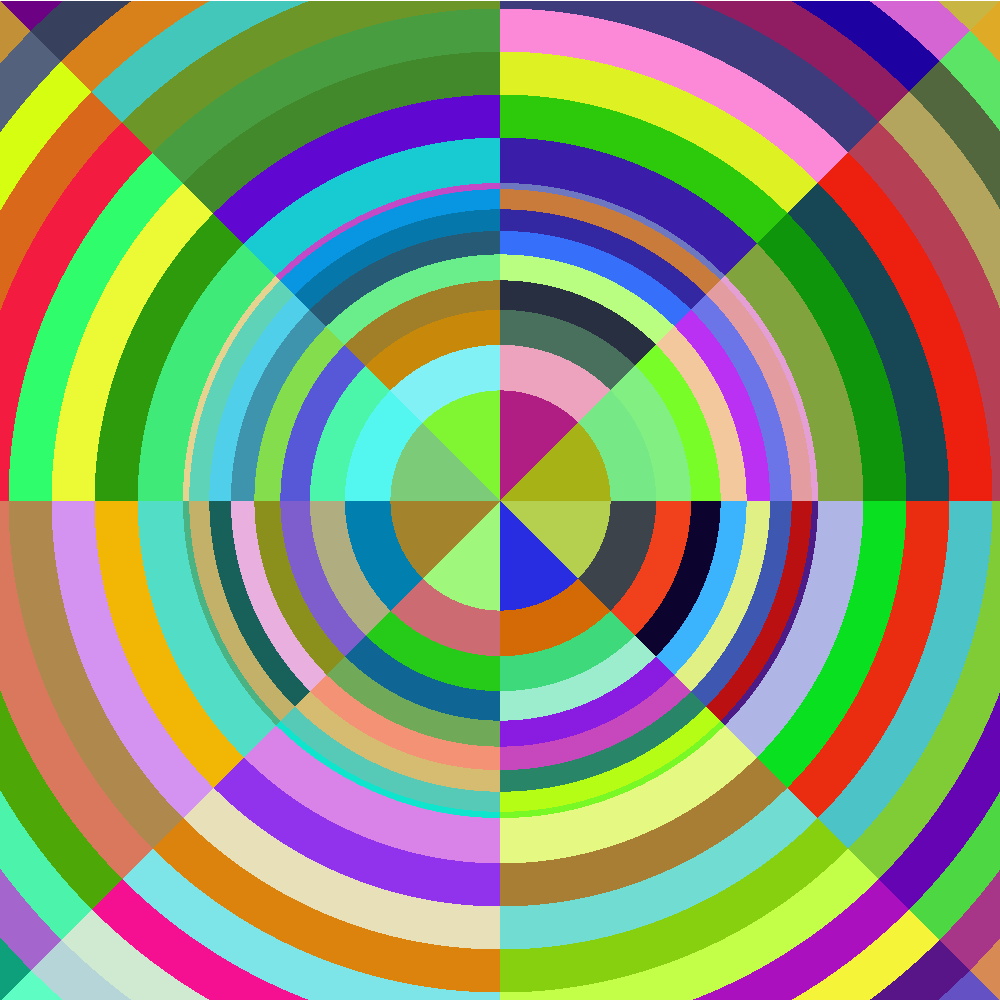
\includegraphics[width=0.9\linewidth]{figures/biases/pin-cell/pin-cell-8x8}
  \caption{}
\end{subfigure}
\caption[Pin cell materials and geometry]{A PWR fuel pin cell with fuel, gap, clad and moderator (a). Radial tally zones were defined in each material in OpenMC (b). The tally zones were further subdivided into angular sectors for the \ac{FSR} mesh in OpenMOC (c).}
\label{fig:chap4-pin-cell}
\end{figure}

The reference eigenvalues computed with continuous energy cross sections in OpenMC are shown in Table~\ref{table:chap4-pin-reference} for both normal anisotropic as well as ``iso-in-lab'' scattering. The reference calculations were computed for 100 batches of 1E7 particles per batch. The reference eigenvalues for the two cases vary by 65 pcm due to anisotropic thermal scattering in the moderator, significantly less than in the 1D slab geometry. The \texttt{openc.mgxs} module was used to compute 70-group libraries of $\Sigma^T_g$, $\Sigma^{Tr}_g$, $\nu\Sigma^F_g$, $\nu_s\Sigma^S_{gg'}$ and $\chi_g$ from OpenMC tallies. An installation of OpenMOC compiled with double precision floating point arithmetic was used for each deterministic simulation. In each calculation, OpenMOC was converged to a criterion of 1E-7 on the energy-integrated fission source.

\begin{table}[h!]
  \centering
  \caption[Reference $k^{OpenMC}_{eff}$ for a 2D fuel pin]{Reference $k^{OpenMC}_{eff}$ for a 2D fuel pin.}
  \label{table:chap4-pin-reference} 
  \vspace{6pt}
  \begin{tabular}{c c}
  \toprule
  \rowcolor{lightgray}
  {\bf Anisotropic} &
  {\bf Isotropic in Lab} \\
  \midrule
  1.17486 $\pm$ 0.00003 & 1.17421 $\pm$ 0.00002 \\
  \bottomrule
\end{tabular}
\end{table}

Table~\ref{table:chap4-pin-angle} presents the bias $\Delta\rho$ for a matrix of azimuthal angles and track spacings. No transport correction was applied to the total cross section $\Sigma^T_g$ or the scattering matrix $\nu_s\Sigma^S_{gg'}$. A single radial tally zone was applied to each material for the \ac{MGXS} calculation with OpenMC. The fuel and moderator were each discretized into 5 equal volume radial rings, and each material zone was discretized into 8 angular sectors for the \ac{FSR} mesh in OpenMOC. The results for both normal anisotropic scattering and ``iso-in-lab'' scattering exhibit a few hundred pcm bias which appears to converge with 128 azimuthal angles and is largely invariant with the track spacing. The \ac{MGXS} tallied with ``iso-in-lab'' scattering in OpenMC converge to an eigenvalue that is roughly 95 pcm less than that computed for the anisotropic case, with a bias of approximately -170 pcm.

\begin{table}[h!]
  \centering
  \caption[Angular discretization error for a 2D fuel pin]{Convergence study of the eigenvalue bias $\Delta\rho$ with varying azimuthal angle quadratures and track spacings for a 2D fuel pin.}
  \label{table:chap4-pin-angle}
  \vspace{6pt}
  \begin{tabular}{a S[table-format=2.1] S[table-format=2.1] S[table-format=2.1] c S[table-format=2.1] S[table-format=2.1] S[table-format=2.1]} 
  \toprule
  \rowcolor{lightgray}
  & \multicolumn{7}{c}{\boldmath $\Delta\rho$ {\bf [pcm]}} \\
  \midrule
  \rowcolor{lightgray}
  {\bf \# Angles} &
  {\bf 0.1 cm} & 
  {\bf 0.01 cm} & 
  {\bf 0.001 cm} &
  &
  {\bf 0.1 cm} & 
  {\bf 0.01 cm} & 
  {\bf 0.001 cm} \\
  \midrule
  & \multicolumn{3}{c}{\cellcolor{carolinablue} \bf Anisotropic} &
  \multicolumn{1}{c}{} &
  \multicolumn{3}{c}{\cellcolor{lightgreen} \bf Isotropic in Lab} \\
4 & 372 & 425 & 427 & & 467 & 519 & 521 \\
8 & -377 & -419 & -418 & & -282 & -325 & -323 \\
16 & -436 & -408 & -412 & & -341 & -314 & -318 \\
32 & -324 & -338 & -331 & & -230 & -244 & -236 \\
64 & -256 & -296 & -285 & & -162 & -202 & -191 \\
128 & -285 & -276 & -267 & & -190 & -182 & -173 \\
256 & -277 & -267 & -265 & & -182 & -173 & -171 \\
512 & -273 & -263 & -264 & & -179 & -169 & -170 \\
  \bottomrule
\end{tabular}
\end{table}

Table~\ref{table:chap4-pin-energy} presents the bias $\Delta\rho$ between OpenMC and OpenMOC for a matrix of energy group structures and \ac{FSR} spatial discretizations. In each case, the \ac{MGXS} used in OpenMOC were tallied by material in OpenMC. The OpenMOC calculations used 128 azimuthal angles and 0.01 cm track spacing. Each of the materials in the fuel pin was discretized into 8 angular sectors. The fuel and moderator were each discretized into 1 -- 16 equal volume radial rings. 

\begin{itemize}[noitemsep]
  \item refer back to figure (a) and (b) for energy/space table
\end{itemize}

\begin{table}[h!]
  \centering
  \caption[Energy and spatial discretization error for a 2D fuel pin]{Convergence study of the eigenvalue bias $\Delta\rho$ with varying energy groups structures and \ac{FSR} spatial discretizations for a 2D fuel pin with \textit{\ac{MGXS} tallied by material}.}
  \label{table:chap4-pin-energy} 
  \vspace{6pt}
  \begin{tabular}{a S[table-format=6.1] S[table-format=6.1] S[table-format=6.1] S[table-format=6.1] S[table-format=6.1]}
  \toprule
  \rowcolor{lightgray}
  & \multicolumn{5}{c}{\boldmath $\Delta\rho$ {\bf [pcm]}} \\
  \midrule
  \rowcolor{lightgray}
  {\textbf{\# Groups}} &
  {\bf 1$\times$} &
  {\bf 2$\times$} &
  {\bf 4$\times$} &
  {\bf 8$\times$} &
  {\bf 16$\times$} \\
  \midrule
  \multicolumn{6}{c}{\cellcolor{carolinablue} \bf Anisotropic $\left(\Sigma^T_g\right)$} \\
1 & 65 & 66 & 66 & 66 & 66 \\
2 & 21 & -23 & -54 & -65 & -64 \\
4 & -60 & -100 & -129 & -143 & -151 \\
8 & -77 & -137 & -183 & -204 & -215 \\
16 & -74 & -141 & -194 & -219 & -230 \\
25 & -130 & -194 & -245 & -272 & -281 \\
40 & -133 & -201 & -257 & -286 & -296 \\
70 & -134 & -204 & -263 & -294 & {\cellcolor{darktangerine}} -304 \\
  \multicolumn{6}{c}{\cellcolor{lightgreen} \bf Anisotropic $\left(\Sigma^{Tr}_g\right)$} \\
1 & 51 & 52 & 52 & 52 & 51 \\
2 & 35 & 6 & -13 & -19 & -11 \\
4 & -60 & -89 & -109 & -125 & -126 \\
8 & -76 & -123 & -158 & -181 & -184 \\
16 & -69 & -124 & -165 & -192 & -196 \\
25 & -126 & -180 & -223 & -249 & -252 \\
40 & -131 & -190 & -239 & -267 & -271 \\
70 & -133 & -194 & -246 & -276 & {\cellcolor{darktangerine}} -280 \\
  \multicolumn{6}{c}{\cellcolor{lightsalmonpink} \bf Isotropic in Lab $\left(\Sigma^T_g\right)$} \\
1 & 79 & 80 & 80 & 80 & 80 \\
2 & 140 & 96 & 65 & 53 & 55 \\
4 & 26 & -14 & -43 & -57 & -65 \\
8 & 25 & -35 & -81 & -102 & -113 \\
16 & 34 & -33 & -86 & -110 & -122 \\
25 & -32 & -95 & -147 & -173 & -182 \\
40 & -39 & -107 & -163 & -192 & -202 \\
70 & -40 & -110 & -169 & -199 & {\cellcolor{darktangerine}} -210 \\
  \bottomrule
\end{tabular}
\end{table}

As was demonstrated for the 1D slab, the results for the fuel pin indicate a strong interaction between the energy and spatial discretization. The eigenvalue bias exhibits a swing of $\sim$350 pcm between energy and spatial meshes. The bias exceeds 200 pcm for all scattering approximations. The application of the transport correction only reduces the bias by up to 25 pcm depending on the energy group structure. The use of the ``iso-in-lab'' scattering feature reduces the bias by roughly $\nicefrac{1}{3}$ or 100 pcm. As was observed for the 1D slab, the bias is negative for all scattering approximations. 

Table~\ref{table:chap4-pin-space} presents the bias for a matrix of energy group structures and \ac{MGXS} spatial tally zone meshes. In each case, the \ac{MGXS} were tallied on the \ac{FSR} mesh used in OpenMOC with 1 -- 16 equal volume rings per material. The OpenMOC calculations used 128 azimuthal angles and 0.01 cm track spacing.

\begin{table}[h!]
  \centering
  \caption[Spatial homogenization error for a 2D fuel pin]{Convergence study of the eigenvalue bias $\Delta\rho$ with varying energy groups structures and \ac{FSR} spatial discretizations for a 2D fuel pin with \textit{\ac{MGXS} tallied by \ac{FSR}}.}
  \label{table:chap4-pin-space} 
  \vspace{6pt}
  \begin{tabular}{a S[table-format=6.1] S[table-format=6.1] S[table-format=6.1] S[table-format=6.1] S[table-format=6.1]}
  \toprule
  \rowcolor{lightgray}
  & \multicolumn{5}{c}{\boldmath $\Delta\rho$ {\bf [pcm]}} \\
  \midrule
  \rowcolor{lightgray}
  {\textbf{\# Groups}} &
  {\bf 1$\times$} &
  {\bf 2$\times$} &
  {\bf 4$\times$} &
  {\bf 8$\times$} &
  {\bf 16$\times$} \\
  \midrule
  \multicolumn{6}{c}{\cellcolor{carolinablue} \bf Anisotropic $\left(\Sigma^T_g\right)$} \\
1 & 67 & 60 & 63 & 98 & 92 \\
2 & 22 & -27 & -56 & -55 & -51 \\
4 & -58 & -101 & -128 & -128 & -135 \\
8 & -75 & -139 & -182 & -194 & -197 \\
16 & -73 & -142 & -190 & -209 & -207 \\
25 & -128 & -198 & -246 & -271 & -268 \\
40 & -131 & -209 & -261 & -288 & -288 \\
70 & -132 & -214 & -267 & -296 & {\cellcolor{darktangerine}} -297 \\
  \multicolumn{6}{c}{\cellcolor{lightgreen} \bf Anisotropic $\left(\Sigma^{Tr}_g\right)$} \\
1 & 53 & 61 & 75 & 66 & 72 \\
2 & 37 & 11 & 1 & -10 & 4 \\
4 & -58 & -83 & -92 & -114 & -109 \\
8 & -74 & -117 & -145 & -175 & -170 \\
16 & -67 & -118 & -154 & -186 & -183 \\
25 & -124 & -181 & -221 & -253 & -245 \\
40 & -130 & -191 & -238 & -272 & -265 \\
70 & -131 & -196 & -245 & -281 & {\cellcolor{darktangerine}} -274 \\
  \multicolumn{6}{c}{\cellcolor{lightsalmonpink} \bf Isotropic in Lab $\left(\Sigma^T_g\right)$} \\
1 & 80 & 92 & 55 & 83 & 66 \\
2 & 141 & 87 & 29 & 50 & 34 \\
4 & 27 & -15 & -43 & -45 & -57 \\
8 & 26 & -34 & -85 & -90 & -102 \\
16 & 35 & -35 & -91 & -101 & -111 \\
25 & -31 & -105 & -158 & -170 & -182 \\
40 & -38 & -114 & -174 & -189 & -202 \\
70 & -39 & -117 & -182 & -196 & {\cellcolor{darktangerine}} -211 \\
  \bottomrule
\end{tabular}
\end{table}

The trends analyzed in Table~\ref{table:chap4-pin-energy} emerge in a similar manner with spatially-dependent \ac{MGXS}. In particular, the eigenvalue bias grows in magnitude with more energy groups and \ac{FSR}s but is largely insensitive to the the elimination of the isotropic scattering approximation. As was observed for the 1D slab, the overall systematic error between OpenMC and OpenMOC is not resolved and in fact increases with greater spatial resolution of the \ac{MGXS}. The results in Table~\ref{table:chap4-pin-space} indicate that spatial self-shielding effects captured with spatially-varying scalar flux-weighted MGXS for each FSR do not have a substantial impact on the systematic errors in the eigenvalue.

%The eigenvalues for the fine energy and spatial mesh are $\sim$60 pcm less than those computed with \ac{MGXS} tallied by material, increasing the magnitude of the bias $\Delta\rho$ by the same amount. The results in Table~\ref{table:chap4-pin-space} demonstrate that spatial self-shielding effects captured with spatially-varying scalar flux-weighted \ac{MGXS} for each \ac{FSR} has a larger impact (60 pcm) than was the case for the 1D slab. However, the overall systematic error between OpenMC and OpenMOC is not resolved and in fact increases with greater spatial resolution of the \ac{MGXS}.


%%%%%%%%%%%%%%%%%%%%%%%%%%%%%%%%%%%%%%%%%%%
%\subsection{2D Fuel Assembly}


%%%%%%%%%%%%%%%%%%%%%%%%%%%%%%%%%%%%%%%%%%%%%%%%%%%%%%%%%%%%%%%%%%%%%%%%%%%%%%%%
\section{Diagnosing the Error}
\label{sec:chap4-diagnosis}

The emergence of a negative systematic bias in the eigenvalue with fine energy and spatial discretization for the heterogeneous 1D slab and 2D fuel pin models led to an analysis of the flux spectra computed by OpenMC and OpenMOC. The 70-group volume-averaged flux in energy for both benchmarks is illustrated in Figure~\ref{fig:chap4-flux}. Upon further inspection, it was noted that OpenMOC's flux exhibited large errors with respect to the reference OpenMC flux in those energy groups which isolate large U-238 capture resonances. The error in the 70-group flux is illustrated in Figure~\ref{fig:chap4-rel-err-energy} for the \ac{FSR}s nearest and furthest from the moderator for the benchmark models with a 16$\times$ \ac{FSR} discretization. Figure~\ref{fig:chap4-rel-err-space} highlights the spatial dependence of the error in group 27 across the fuel which isolates the largest U-238 capture resonance at 6.67 eV. For both the slab and the fuel pin the error monotonically decreases from a maximum of more than 2\% to a minimum of $\sim$-0.3\% in those \ac{FSR}s furthest and nearest the moderator, respectively. 

\begin{itemize}[noitemsep]
  \item Only plot the flux in the fuel
  \item Add footnote making mention of the closeness between OpenMC/MOC
\end{itemize}

\begin{figure}[H]
\begin{subfigure}{0.9\textwidth}
  \centering
  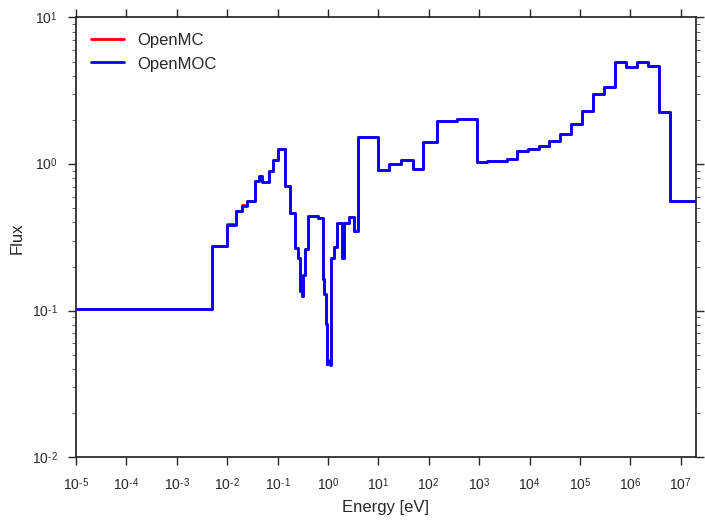
\includegraphics[width=\linewidth]{figures/biases/slab/vol-avg-flux}
  \caption{}
\end{subfigure}
\begin{subfigure}{0.9\textwidth}
  \centering
  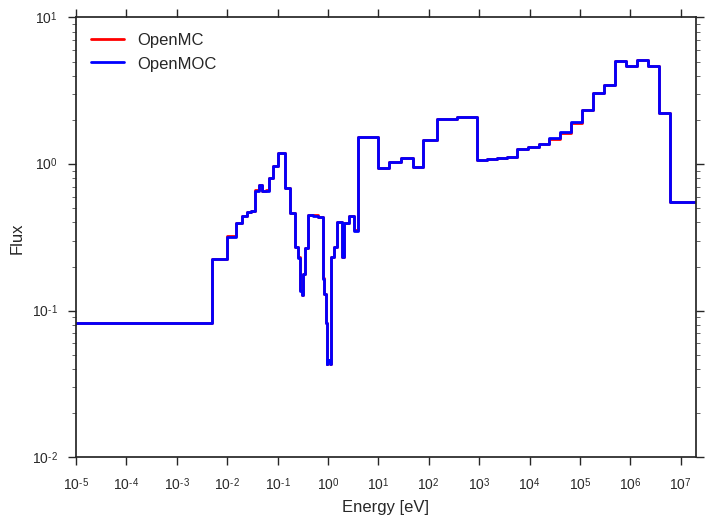
\includegraphics[width=\linewidth]{figures/biases/pin-cell/vol-avg-flux}
  \caption{}
\end{subfigure}
\caption[Flux spectrum in a slab and pin cell]{The flux spectrum in energy in a 1D slab (a) and 2D fuel pin (b).}
\label{fig:chap4-flux}
\end{figure}

\begin{figure}[H]
\begin{subfigure}{.9\textwidth}
  \centering
  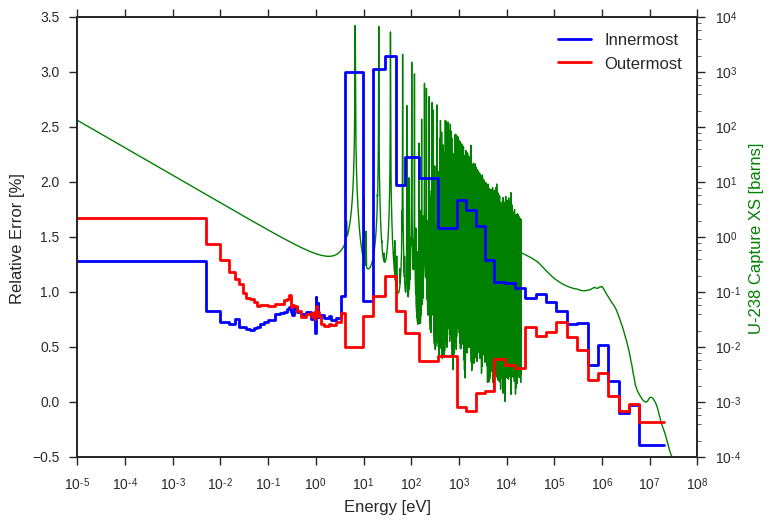
\includegraphics[width=\linewidth]{figures/biases/slab/rel-err-inner-outer}
  \caption{}
\end{subfigure}
\begin{subfigure}{.9\textwidth}
  \centering
  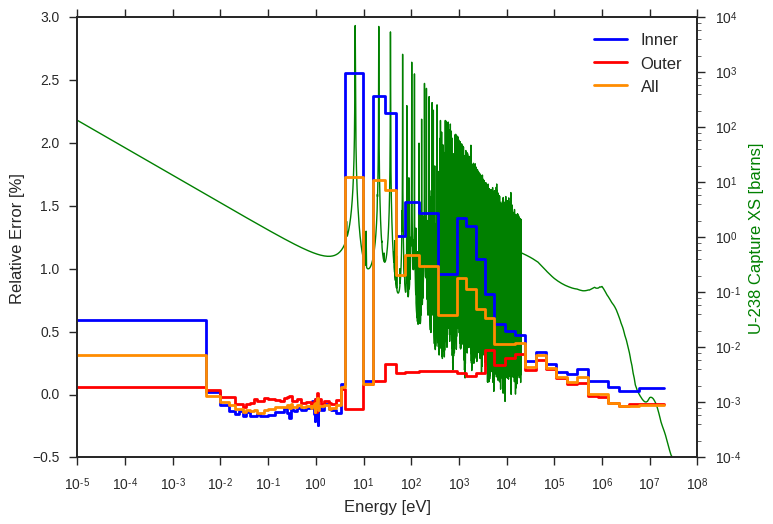
\includegraphics[width=\linewidth]{figures/biases/pin-cell/rel-err-inner-outer}
  \caption{}
\end{subfigure}
\caption[Flux relative error by energy group]{The energy-dependent relative error of the OpenMOC scalar flux with respect to the reference OpenMC flux for a 1D slab (a) and 2D fuel pin (b). The results correspond to Tables~\ref{table:chap4-slab-space} and~\ref{table:chap4-pin-space} for \ac{MGXS} tallied on a 16$\times$ \ac{FSR} mesh with ``iso-in-lab'' scattering. The errors are illustrated for the innermost and outermost fuel \ac{FSR}s.}
\label{fig:chap4-rel-err-energy}
\end{figure}

\begin{itemize}[noitemsep]
  \item Add group to the figure of spatially-varying error
  \item Add spatially-varying error for Ranges A, B and C to each plot
\end{itemize}

\begin{figure}[H]
\begin{subfigure}{.9\textwidth}
  \centering
  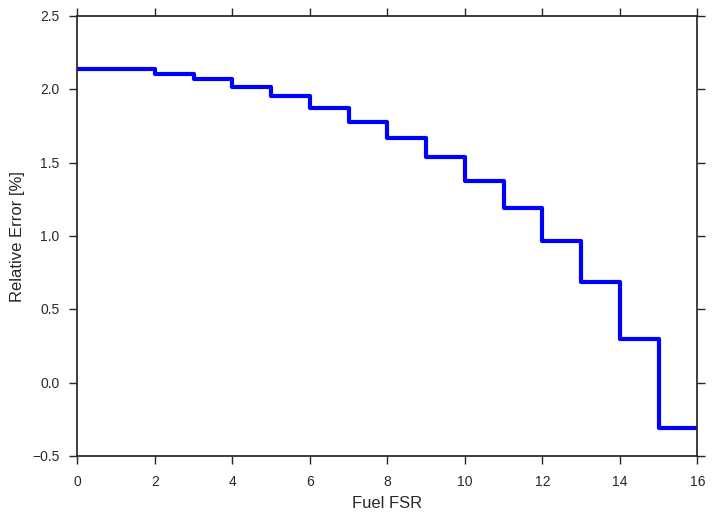
\includegraphics[width=\linewidth]{figures/biases/slab/rel-err-fuel-fsrs}
  \caption{}
\end{subfigure}
\begin{subfigure}{.9\textwidth}
  \centering
  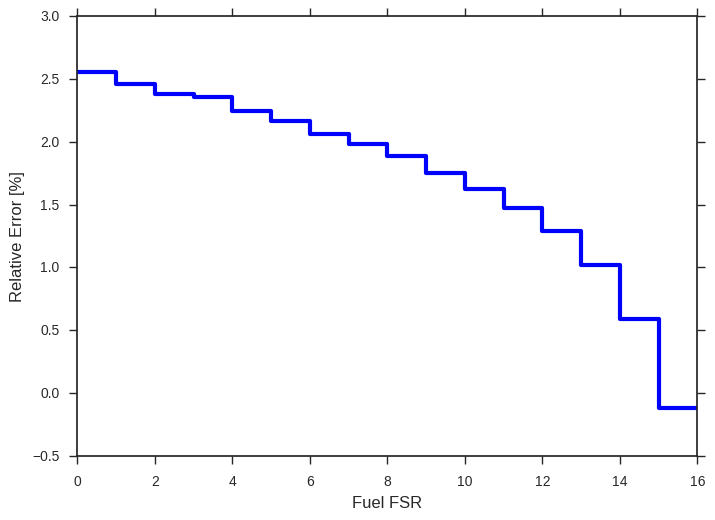
\includegraphics[width=\linewidth]{figures/biases/pin-cell/rel-err-fuel-fsrs}
  \caption{}
\end{subfigure}
\caption[Flux relative error by FSR]{The spatially-varying relative error of the OpenMOC scalar flux with respect to the reference OpenMC flux for a 1D slab (a) and 2D fuel pin (b). The results correspond Tables~\ref{table:chap4-slab-space} and~\ref{table:chap4-pin-space} for \ac{MGXS} tallied on a 16$\times$ \ac{FSR} mesh with ``iso-in-lab'' scattering. The errors are plotted for each of the 16 \ac{FSR}s in the fuel.}
\label{fig:chap4-rel-err-space}
\end{figure}

The errors in the multi-group flux directly correspond to equal errors in the reaction rates since the \ac{MGXS} are computed from the reference reaction rate and flux tallies. The results presented in Figure~\ref{fig:chap4-rel-err-energy} indicate significant errors in resonance groups, and in particular, group 27 in the 70-group calculation. The percent relative error for both U-238 capture and total absorption for all nuclides is quantified in Table~\ref{table:chap4-rxn-rate-errors} for different energy regimes. Each of the columns corresponds to the reaction rate errors in the following energy ranges:

\vspace{-0.1in}
\begin{itemize}[noitemsep]
  \item {\bf Range A} -- group encompassing the U-238 capture resonance at 6.67 eV
  \item {\bf Range B} -- groups encompassing the resonace range from 4 eV -- 200 keV
  \item {\bf Range C} -- groups encompassing the entire energy regime from 0 -- 20 MeV
\end{itemize}
\vspace{-0.1in}

As illustrated in the table, both U-238 capture and total absorption rate error grows with the number of energy groups used in the \ac{MGXS} calculation. This trend is particularly pronounced for U-238 capture in the 6.67 eV resonance group which exceeds 1\% when 25 or more groups are used in the multi-group calculation. The 0.1\% and 0.17\% error in the total absorption would directly correspond to an under-prediction in the eigenvalue of 115 and 197 pcm for the slab and fuel pin, respectively, which closely matches the observed eigenvalue biases for each model\footnote{This analysis neglects the contribution of scattering multiplicity (\textit{e.g.,} (n,xn)) to the eigenvalue.}. Approximately 5 -- 6\% and 16 -- 18\% of the total absorption occurs in energy ranges A and B, with U-238 capture accounting for 80\% and 70\% of the total absorption in each energy range, respectively. Hence, the error in U-238 resonance capture alone would under-predict the eigenvalue by 105 and 145 pcm for the slab and pin, with approximately half of the error deriving from group 27 of 70 due to the resonance at 6.67 eV. 

%U-238 capture
%slab 27: 50 pcm
%slab all: 105 pcm
%pin 27: 100 pcm
%pin all: 185 pcm

%The total energy-integrated fission rate error is $\sim$1\% and $\sim$0.25\% for the slab and pin (and over 2\% in group 27) which would correspond to an over-prediction in the eigenvalue of

%Taken together, the errors in the absorption and fission rates would result in an eigenvalue bias that compares closely with the observed $\Delta\rho \approx$ 300 -- 350 pcm \footnote{This analysis neglects the contribution of scattering multiplicity (\textit{e.g.,} (n,2n)) to the eigenvalue.}.

%Figure~\ref{fig:chap4-pin-fuel-fsrs} highlights the spatial dependence of the error in group 27 across the fuel which isolates the largest U-238 capture resonance at 6.67 eV. The error decreases from a maximum of $\sim$2.8\% to a minimum of $\sim$0.6\% in those \ac{FSR}s furthest and nearest the moderator, respectively. It is unclear why the spatial dependence of the error does not monotonically decrease across the fuel pin as it does for the slab (see Figure~\ref{fig:chap4-slab-fuel-fsrs}), but the overall trend is the same.

{\setlength{\extrarowheight}{-5pt}
\begin{table}[H]
  \centering
  \caption[Reaction rate relative errors]{The volume-integrated U-238 capture and total absorption rate percent relative error for a 1D slab and 2D fuel pin. The error correspond to the results in Tables~\ref{table:chap4-slab-space} and \ref{table:chap4-pin-space} for \ac{MGXS} tallied on a 16$\times$ \ac{FSR} mesh with ``iso-in-lab'' scattering.}
  \small
  \label{table:chap4-rxn-rate-errors} 
  \vspace{6pt}
  \begin{tabular}{a S[table-format=6.1] S[table-format=6.1] S[table-format=6.1] c S[table-format=6.1] S[table-format=6.1] S[table-format=6.1]}
  \toprule
  \rowcolor{lightgray}
  \multicolumn{1}{c}{\bf \# Groups} &
  \multicolumn{3}{c}{\bf U-238 Capture} &
  \multicolumn{1}{c}{} &
  \multicolumn{3}{c}{\bf Total Absorption} \\
  \midrule
  \multicolumn{8}{c}{\cellcolor{carolinablue} \bf 1D Slab} \\
  & {\bf \cellcolor{lightgray} Range A} &
  {\bf \cellcolor{lightgray} Range B} &
  {\bf \cellcolor{lightgray} Range C} &
  &
  {\bf \cellcolor{lightgray} Range A} &
  {\bf \cellcolor{lightgray} Range B} &
  {\bf \cellcolor{lightgray} Range C} \\
1 & -0.03 & -0.03 & -0.03 & & -1.58 & -1.58 & -1.58 \\
2 & 1.17 & 1.17 & 0.66 & & 1.03 & 1.03 & -0.43 \\
4 & -0.18 & 0.23 & -0.07 & & -0.17 & 0.22 & -0.44 \\
8 & 0.20 & 0.53 & 0.13 & & 0.23 & 0.52 & -0.14 \\
16 & 0.25 & 0.58 & 0.16 & & 0.28 & 0.57 & -0.09 \\
25 & 0.61 & 0.35 & 0.21 & & 0.64 & 0.37 & -0.08 \\
40 & 0.63 & 0.44 & 0.25 & & 0.66 & 0.45 & -0.05 \\
70 & {\cellcolor{darktangerine}} 0.64 & 0.48 & 0.26 & & 0.67 & 0.49 & -0.04 \\
%1 & -0.02 & -0.02 & -0.02 & & -0.52 & -0.52 & -0.52 \\
%2 & 0.48 & 0.48 & 0.30 & & 0.45 & 0.45 & -0.21 \\
%4 & 0.19 & 0.00 & 0.11 & & 0.20 & 0.00 & -0.20 \\
%8 & 0.46 & 0.17 & 0.26 & & 0.49 & 0.17 & -0.03 \\
%16 & 0.50 & 0.21 & 0.28 & & 0.53 & 0.21 & 0.01 \\
%25 & 1.05 & 0.65 & 0.45 & & 1.07 & 0.67 & 0.06 \\
%40 & 1.07 & 0.75 & 0.49 & & 1.09 & 0.76 & 0.09 \\
%70 & {\cellcolor{darktangerine}} 1.07 & 0.81 & 0.50 & & 1.10 & 0.82 & 0.10 \\
  \multicolumn{8}{c}{\cellcolor{lightgreen} \bf 2D Fuel Pin} \\
  & {\bf \cellcolor{lightgray} Range A} &
  {\bf \cellcolor{lightgray} Range B} &
  {\bf \cellcolor{lightgray} Range C} &
  &
  {\bf \cellcolor{lightgray} Range A} &
  {\bf \cellcolor{lightgray} Range B} &
  {\bf \cellcolor{lightgray} Range C} \\
1 & -0.02 & -0.02 & -0.02 & & -0.07 & -0.07 & -0.07 \\
2 & 0.11 & 0.11 & 0.07 & & 0.11 & 0.11 & -0.03 \\
4 & 0.55 & 0.07 & 0.32 & & 0.54 & 0.07 & 0.04 \\
8 & 0.71 & 0.11 & 0.40 & & 0.72 & 0.11 & 0.08 \\
16 & 0.72 & 0.12 & 0.41 & & 0.73 & 0.12 & 0.09 \\
25 & 1.32 & 0.85 & 0.61 & & 1.34 & 0.85 & 0.15 \\
40 & 1.33 & 0.93 & 0.64 & & 1.34 & 0.92 & 0.16 \\
70 & {\cellcolor{darktangerine}} 1.33 & 0.99 & 0.65 & & 1.35 & 0.97 & 0.17 \\
  \bottomrule
\end{tabular}
\end{table}}

These results indicate that spatial self-shielding effects in resonance groups is not adequately captured by the \ac{MGXS} and/or the multi-group calculation. Furthermore, this analysis illustrates the counter intuitive result that the bias between continuous energy Monte Carlo and multi-group deterministic transport may in fact increase in magnitude with more energy groups. Although it is challenging to isolate the factors which convolve to bias the eigenvalue, the data presented here indicates that an over-prediction of U-238 capture in the resonance groups largely drives the error. These results will be discussed in greater depth in the context of angular-dependent \ac{MGXS} in Chapter~\ref{chap:sph}.